\documentclass[12pt]{article}

% ========= Packages =========
\usepackage{geometry}
\usepackage{setspace}
\usepackage{amsmath,amssymb,amsthm}
\usepackage{booktabs}
\usepackage{siunitx}
\usepackage{textcomp}
\usepackage{graphicx}
\usepackage{threeparttable}
\usepackage[round]{natbib}
\usepackage{hyperref}
\usepackage{xcolor}
\usepackage{tikz}
\usetikzlibrary{patterns,arrows.meta,positioning}
\usepackage[font=small,labelfont=bf,labelsep=period,skip=6pt]{caption}

\hypersetup{colorlinks=true,linkcolor=blue,citecolor=blue,urlcolor=blue}

% ========= Page and layout =========
\geometry{margin=1in}
\doublespacing
\setlength{\parindent}{0.5in}
\raggedbottom
\clubpenalty=10000
\widowpenalty=10000
\displaywidowpenalty=10000
\renewcommand{\textfraction}{0.10}
\renewcommand{\topfraction}{0.90}
\renewcommand{\bottomfraction}{0.80}
\renewcommand{\floatpagefraction}{0.80}
\setcounter{topnumber}{3}
\setcounter{bottomnumber}{2}
\setcounter{totalnumber}{4}
\setlength{\textfloatsep}{10pt plus 2pt minus 2pt}
\setlength{\floatsep}{8pt plus 2pt minus 2pt}
\setlength{\intextsep}{8pt plus 2pt minus 2pt}
\setlength{\abovecaptionskip}{4pt}
\setlength{\belowcaptionskip}{0pt}

% ========= Math & units =========
\numberwithin{equation}{section}
\sisetup{
  detect-mode = true,
  table-number-alignment = center,
  input-exponent-markers = e,
  group-separator = {,}
}
\DeclareSIUnit{\milliSecond}{ms}
\DeclareSIUnit{\dollar}{\$}
\DeclareSIUnit{\billion}{B}
\DeclareSIUnit{\percent}{\%}
\DeclareSIUnit{\cent}{\textcent}

% ========= Macros =========
\newcommand{\QOU}{\mathrm{QOU}}
\newcommand{\LCI}{\mathrm{LCI}}
\newcommand{\IPD}{\mathrm{IPD}}
\newcommand{\E}{\mathbb{E}}
\newcommand{\Prb}{\mathbb{P}}
\newcommand{\elloc}{\mathrm{loc}}

\begin{document}

% ================= Title =================
\begin{center}
{\LARGE \textbf{The Cost of Usable Intelligence: Measuring AI’s Economic Productivity Frontier}}

\vspace{0.6cm}
\textbf{Aditya Morey}\\[4pt]
\small{[Affiliation Redacted for Draft]}\\[4pt]
\small{Corresponding author: [CONTACT INFO REDACTED]}\\[8pt]
\end{center}

% ================= Executive Summary =================
\noindent\textbf{Executive Summary}  

\noindent Intelligence is becoming a traded input. Yet we lack a coherent price for it.  
This paper defines the \emph{Locational Cost of Intelligence} (LCI): the minimum cost to deliver one usable unit of AI output at specified accuracy, latency, reliability, and safety (QoS).  
We treat QoS as chance-constrained production, grounded in queueing and neural scaling, and aggregate with a chain Fisher \emph{Intelligence Price Deflator} (IPD).  
The framework quantifies architecture choices (RAG vs.\ scale) and shows how energy and transmission reshape the geography of AI productivity.

\vspace{0.6em}
\noindent\textbf{Keywords:} AI economics; hedonic price index; queueing; service level objectives; infrastructure policy

\newpage

% ================= Abstract =================
\noindent\textbf{Abstract}  

\noindent We define the \emph{Locational Cost of Intelligence} (LCI): the dual cost of producing one task-equivalent unit of AI output at targeted accuracy, latency, reliability, and safety under a joint probabilistic constraint.  
We formalize serving using GI/G/$k$ with processor sharing and batching, provide tractable surrogates for the chance constraint, and construct a chain Fisher \emph{Intelligence Price Deflator} (IPD).  
A public-data calibration illustrates how retrieval depth substitutes for model scale and how transmission lowers LCI on both energy and latency margins.  
This reframes AI’s macro impact as changes in the price of \emph{usable} intelligence.

\vspace{0.3cm}
\noindent\textbf{JEL Codes:} D24, L11, O33

\newpage

% ================= 1. Introduction =================
\section{Introduction and Motivation}

Economic measurement should price what firms \emph{sell}: usable, quality-guaranteed completions, not raw tokens or GPU-hours.  
We define the \emph{Locational Cost of Intelligence} (LCI) as the minimum cost to produce one task-equivalent unit at QoS thresholds, conditional on local factor prices.  
LCI is task-family specific, QoS-constrained, and location-aware.

\paragraph{Bridge.}
Hedonic methods priced quality-adjusted IT capital \citep{Triplett1989,Pakes2003,Byrne2017}.  
LCI prices quality-adjusted AI services, integrating accuracy, latency, reliability, and safety into a single cost object.  
Intelligence becomes measurable—comparable across architectures and geographies.

\paragraph{Notation.}
Inputs $x=(H,P,W,N,O)$ denote hardware capacity, power, labor, network, and orchestration; prices $p=(\kappa_K,c_E,w,c_N,\dots)$ are location-specific.  
Scale $m$, retrieval depth $R$, and tooling $Z$ shape accuracy; load $u\in[0,u_{\max})$ drives tail latency.

% ============ Figure 1: Stylized LCI vs QoS frontier ============
\begin{figure}[t]
\centering
\begin{tikzpicture}[x=1cm,y=1cm,>=Latex]
  \draw[->] (0,0) -- (9.2,0) node[below right]{QoS composite ($a\uparrow,\ \ell\downarrow,\ q\uparrow,\ s\uparrow$)};
  \draw[->] (0,0) -- (0,5.0) node[above left]{LCI (cost per usable task)};
  % Frontier curve (convex, diminishing improvement)
  \draw[thick,blue,smooth] plot coordinates {
    (0.7,4.2) (1.4,3.5) (2.2,2.8) (3.2,2.2) (4.2,1.8) (5.2,1.55) (6.2,1.40) (7.2,1.30) (8.2,1.25)
  };
  \node[blue] at (6.8,1.6) {\small Frontier};
  % Region markers
  \fill[green!60!black] (3.2,2.2) circle (2pt); \node[anchor=west,align=left] at (3.35,2.15) {\scriptsize Virginia};
  \fill[teal!70!black] (4.6,1.9) circle (2pt); \node[anchor=west] at (4.75,1.85) {\scriptsize Texas};
  \fill[orange!80!black] (6.6,1.45) circle (2pt); \node[anchor=west] at (6.75,1.40) {\scriptsize Ireland};
  \fill[red!70!black] (7.6,1.33) circle (2pt); \node[anchor=west] at (7.75,1.29) {\scriptsize Singapore};
\end{tikzpicture}
\caption{Stylized intelligence frontier: LCI falls with better QoS but flattens near limits; location shifts the attainable locus.}
\label{fig:frontier}
\end{figure}

% ================= 2. Framework =================
\section{The LCI Framework}

\subsection{Quality-Adjusted Output (QOU)}
Tokens are intermediate; output is task-equivalent completions with QoS.
\begin{equation}
\QOU = T \cdot \phi(a,\ell,q,s),\qquad
\phi(a,\ell,q,s)=\alpha(a)\,\lambda(\ell)\,\rho(q)\,\sigma(s),
\end{equation}
\begin{align}
\alpha(a)&=a^{\eta_a}, &
\rho(q)&=q^{\eta_q}, &
\sigma(s)&=s^{\eta_s},\\
\lambda(\ell)&=\left(\frac{\bar\ell}{\max(\ell,\bar\ell)}\right)^{\eta_\ell}.
\end{align}
At or below $\bar\ell$ there is no latency penalty; in calibration we use a smooth hinge.

\subsection{Serving and Tail Latency}
Throughput $T$ follows a scale-with-utilization form:
\begin{equation}
T = A_0\,H^{\beta_H} P^{\beta_P} W^{\beta_W} N^{\beta_N} O^{\beta_O}\cdot g(u),\quad
g(u)=\left(1-\frac{u}{u_{\max}}\right)^{\gamma}.
\end{equation}
We use GI/G/$k$ with processor sharing and batching $(B,\tau_b)$.  
Let $W_\alpha$ be the $\alpha$-quantile of response time.  
Heavy-traffic approximations imply $W_{0.95}(u)$ is convex near $u_{\max}$; we map $\ell=W_{0.95}$.

% ============ Figure 2: Queueing throughput & convexity ============
\begin{figure}[t]
\centering
\begin{tikzpicture}[x=1cm,y=1cm,>=Latex]
  % Axes
  \draw[->] (0,0) -- (7.6,0) node[below right]{Utilization $u$};
  \draw[->] (0,0) -- (0,4.6) node[above left]{Throughput / LCI};
  % Throughput curve
  \draw[thick,blue]
    plot[smooth] coordinates {(0.5,3.8) (1.2,3.5) (2.0,3.0) (2.8,2.4) (3.6,1.8) (4.4,1.3) (5.2,0.9) (6.0,0.7) (6.8,0.6)};
  \node[blue] at (1.3,3.95) {\scriptsize $T(u)$};
  % LCI curve (convex near saturation)
  \draw[thick,red]
    plot[smooth] coordinates {(0.5,0.6) (1.3,0.7) (2.1,0.95) (2.9,1.35) (3.7,1.95) (4.5,2.8) (5.3,3.7) (6.1,4.2) (6.9,4.45)};
  \node[red] at (4.9,3.6) {\scriptsize $\LCI(u)$};
  % u_max marker
  \draw[densely dashed] (6.5,0) -- (6.5,4.4);
  \node[below] at (6.5,0) {\scriptsize $u_{\max}$};
\end{tikzpicture}
\caption{Serving class and operating point: $T(u)$ tapers while $\LCI(u)$ becomes convex near saturation due to tail-latency penalties.}
\label{fig:queue}
\end{figure}

\paragraph{Accuracy from scaling.}
Empirical scaling motivates a saturating form:
\begin{equation}
a = 1 - \exp\!\Big[-\big(\theta_m m^{\zeta_m} + \theta_R R^{\zeta_R} + \theta_{mR} m^{\zeta_m}R^{\zeta_R} + \theta_Z Z\big)\Big].
\end{equation}

\subsection{Chance-Constrained Program}
\begin{equation}
\label{eq:program}
\begin{aligned}
\min_{x,u,m,R,Z,B,\tau_b} \quad & C(x;p,\elloc) \\
\text{s.t.} \quad
& \E[\QOU(x,u,m,R,Z)] \ge Q,\\
& \Prb\!\big(a\!\ge\!\bar a,\, \ell\!\le\!\bar\ell,\, q\!\ge\!\bar q,\, s\!\ge\!\bar s\big)\ \ge 1-\varepsilon.
\end{aligned}
\end{equation}
Define $\LCI=c_{\mathcal{T}}(Q;p,\elloc,\varepsilon)/Q$; by Shephard’s lemma, $\partial \LCI/\partial p_j=x_j^*/Q$.

% ================= 3. Properties =================
\section{Properties and Testable Implications}

\paragraph{A. RAG–Scale Efficiency Region.}
At the cost-minimizing allocation,
\[
\frac{\theta_R \zeta_R R^{\zeta_R}}{MC_R/R} >
\frac{\theta_m \zeta_m m^{\zeta_m}}{MC_m/m}
\Rightarrow \text{RAG dominates scale in QOU-per-dollar.}
\]

\paragraph{B. Two-Margin Effect of Transmission.}
Transmission lowers $c_E$ and relaxes latency constraints by enabling relocation, reducing network distance and cooling penalties.

\paragraph{C. Convexity Near Saturation.}
Under GI/G/$k$–PS with batching $(B,\tau_b)$ and finite second moments, $W_{0.95}(u)$ is convex for $u$ near $u_{\max}$; hence $\LCI(u)$ is convex.

% ============ Figure 3: RAG vs Scale map (stylized) ============
\begin{figure}[t]
\centering
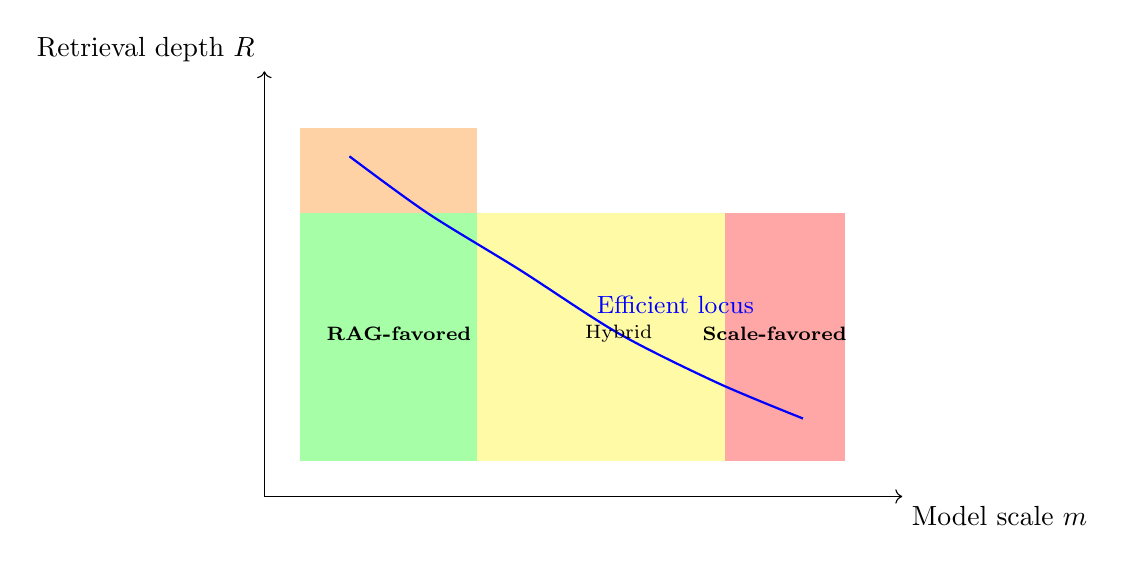
\begin{tikzpicture}[x=0.9cm,y=0.9cm]
  % axes
  \draw[->] (0,0) -- (9,0) node[below right]{Model scale $m$};
  \draw[->] (0,0) -- (0,6) node[above left]{Retrieval depth $R$};
  % heat-style regions (stylized blocks)
  \fill[green!35] (0.5,0.5) rectangle (3.0,4.0);
  \fill[yellow!35] (3.0,0.5) rectangle (6.5,4.0);
  \fill[orange!35] (0.5,4.0) rectangle (3.0,5.2);
  \fill[red!35] (6.5,0.5) rectangle (8.2,4.0);
  % frontier line (qualitative)
  \draw[thick,blue,smooth] plot coordinates {(1.2,4.8) (2.3,4.0) (3.6,3.2) (5.0,2.3) (6.4,1.6) (7.6,1.1)};
  \node[blue] at (5.8,2.7) {\small Efficient locus};
  \node at (1.9,2.3) {\scriptsize \textbf{RAG-favored}};
  \node at (5.0,2.3) {\scriptsize Hybrid};
  \node at (7.2,2.3) {\scriptsize \textbf{Scale-favored}};
\end{tikzpicture}
\caption{Stylized RAG–scale map: at low $MC_R$ and moderate $m$, RAG yields lower LCI; as $MC_m$ falls or $\zeta_m$ rises, scale favorability expands.}
\label{fig:ragscale}
\end{figure}

% ================= 4. Empirical Calibration =================
\section{Empirical Calibration}

\begin{table}[t]
\centering
\begin{threeparttable}
\caption{Empirical primitives (latest available at collection time)}
\label{tab:empirical}
\begin{tabular}{l l l l}
\toprule
Category & Region / Item & Value & Source \\
\midrule
Industrial electricity & Virginia (US) & 9.49~\si{\cent\per\kilo\watt\hour} & EIA Table 5.6.A \\
Industrial electricity & Texas (US) & 6.60~\si{\cent\per\kilo\watt\hour} & EIA Table 5.6.A \\
GPU (H100) price & p5.4xlarge & \$3.93 / accelerator-hour & Cloud price list \\
GPU (8$\times$H100) & p5.48xlarge & \$31.46 / instance-hour & Cloud price list \\
Retrieval (reads) & Vector DB (reads) & \$16 / 1M read units & Provider pricing \\
Retrieval (storage) & Vector DB (storage) & \$0.095 / 1M dims·month & Provider pricing \\
Inter-region latency & us-east-1$\to$eu-west-1 & 70–90~\si{\milliSecond} & Public measurements \\
\bottomrule
\end{tabular}
\end{threeparttable}
\end{table}

% ============ Figure 4: IPD trend (stylized) ============
\begin{figure}[t]
\centering
\begin{tikzpicture}[x=1cm,y=1cm]
  \draw[->] (0,0) -- (9.2,0) node[below right]{Time};
  \draw[->] (0,0) -- (0,5.0) node[above left]{Index (2024Q1=100)};
  % Virginia
  \draw[thick,blue] plot[smooth] coordinates {(0.8,4.5) (2.0,4.2) (3.2,3.9) (4.4,3.6) (5.6,3.4) (6.8,3.2) (8.0,3.1)};
  \node[blue] at (7.2,3.35) {\scriptsize Virginia};
  % Singapore
  \draw[thick,red] plot[smooth] coordinates {(0.8,4.5) (2.0,4.4) (3.2,4.35) (4.4,4.3) (5.6,4.35) (6.8,4.45) (8.0,4.55)};
  \node[red] at (7.2,4.6) {\scriptsize Singapore};
\end{tikzpicture}
\caption{Illustrative IPD series: regions with cheaper energy/transmission exhibit faster declines in the price of usable intelligence.}
\label{fig:ipd}
\end{figure}

% ================= 5. Intelligence Price Deflator =================
\section{Intelligence Price Deflator (IPD)}

Let $\{\mathcal T_k\}$ be task families with shares $s_{k,t}$.  
We compute a chain Fisher across families:
\begin{equation}
\IPD_t
=\prod_{\tau=1}^{t}
\sqrt{
\sum_k s_{k,\tau-1}\frac{\LCI_{k,\tau}}{\LCI_{k,\tau-1}}
\cdot
\sum_k s_{k,\tau}\frac{\LCI_{k,\tau}}{\LCI_{k,\tau-1}}
}.
\end{equation}
We report Laspeyres/Paasche bounds and decompose changes into within-family LCI, between-family shares, and entry/exit.

% ================= 6. Implications =================
\section{Implications}

\textit{Architecture choice.} The RAG–scale map (Fig.~\ref{fig:ragscale}) gives a transparent rule-of-thumb for capacity planning: push toward the region with higher QOU-per-dollar marginal effect.  
\textit{Geography.} Transmission improves LCI via energy \emph{and} latency, shifting optimal location choice.  
\textit{Macro.} IPD tracks real progress in the cost of capability, separating engineering gains from demand noise.

% ================= 7. Limitations =================
\section{Limitations and Conclusion}

QoS targets are fixed within periods; multi-tenancy and heterogeneity are abstracted into capacity reservations; correlations among failure modes are handled via tractable surrogates.  
Even so, LCI provides a durable bridge from engineering primitives to economic measurement, pricing what matters: usable intelligence.

% ================= References =================
\begin{thebibliography}{}
\bibitem[Byrne and Syverson(2017)]{Byrne2017}
Byrne, D. M., and C. Syverson (2017). “Prices, Productivity, and Output in the Digital Economy.” \emph{American Economic Review}, 107(5): 168–172.
\bibitem[Pakes(2003)]{Pakes2003}
Pakes, A. (2003). “A Reconsideration of Hedonic Price Indices with an Application to PCs.” \emph{American Economic Review}, 93(5): 1578–1596.
\bibitem[Triplett(1989)]{Triplett1989}
Triplett, J. E. (1989). “Price and Technological Change in a Capital Good: A Survey of Research on Computers.” \emph{Brookings Papers on Economic Activity: Microeconomics}, 373–438.
\end{thebibliography}

% ================= Appendices =================
\appendix

\section*{Appendix A: Tractable Chance Constraints}

The joint constraint
\[
\Prb\left(a\!\ge\!\bar a,\,\ell\!\le\!\bar\ell,\,q\!\ge\!\bar q,\,s\!\ge\!\bar s\right)\ge 1-\varepsilon
\]
is non-convex in general. Two convex surrogates enable estimation:

\emph{Bonferroni.} Pick $(\varepsilon_a,\varepsilon_\ell,\varepsilon_q,\varepsilon_s)$ with $\sum\varepsilon_i\le\varepsilon$, impose marginals $\Prb(a<\bar a)\le\varepsilon_a$, $\Prb(\ell>\bar\ell)\le\varepsilon_\ell$, etc.  

\emph{CVaR.} Let $L$ aggregate shortfalls; enforce $\mathrm{CVaR}_{\varepsilon}(L)\le 0$, a convex constraint under standard loss constructions.
Both admit polynomial-time solvers for $c_{\mathcal T}$ and comparative statics via the envelope theorem.

\section*{Appendix B: Data and Replication Notes}

Calibration uses public sources (energy, cloud accelerator prices, vector DB pricing, and inter-region latency measurements).  
CSV primitives are versioned in \texttt{results/tables/}; scripts render tables and figures in CI.  
Energy and retrieval data harmonized to common monthly units; latency values reflect p50 inter-region RTTs.

\end{document}
